\section{Pilot Study}

As we see later in Section \ref{section:device-fingerprinting} the efficiency of the methods to clean and aggregate data not only depend on the noise and bias in the data itself but also on external factors such as, the configuration of the sensor in relation to the environment, the day of the week etc.
Thus the dataset captured in our initial experiments, though acts as a good starting point, cannot enable us to generalise our findings to all possible configurations.
This necessitates an even larger data collected over longer durations in challenging situations we usually find in real world conditions.
This was our primary motivation in conducting a pilot study collecting data at 5 locations across London.
The aim was to collect probe requests with information we found relevant in the initial experiments for every location surveyed for at least a full week so that we can understand any artifacts caused by the periodicity of the data.
We also wanted to collect data at all these locations in parallel for at least a week so that they can be compared to one other. 

\subsection{Methodology}

\begin{marginfigure}[2cm]
  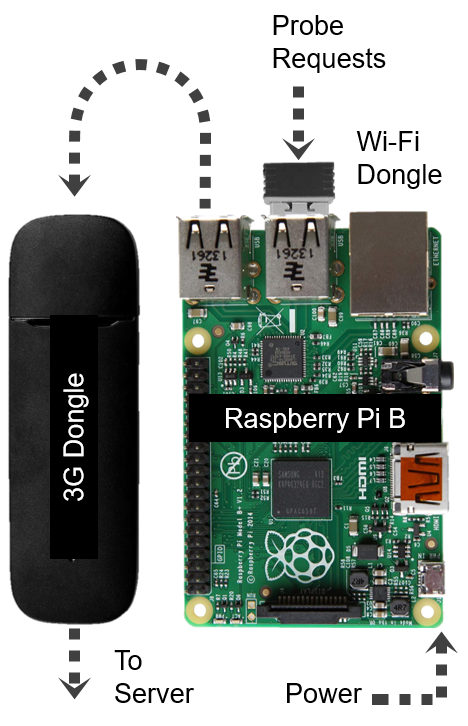
\includegraphics{images/pilot-hardware.png}
  \caption{Hardware setup used to collect data in the pilot studies.}
  \label{figure:collection:pilot:hardware}
\end{marginfigure}

The hardware setup for the sensors is illustrated in Figure \ref{figure:collection:pilot:hardware}.
It design of the hardware is not original as it is heavily influenced by the proprietary technology of the data partner for the Smart Street Sensor project albeit a much simpler form. 
The core of the hardware is the general purpose single board computer - Raspberry Pi Model B running Linux Operating system.
Two communication modules - 3G and Wi-Fi were connected to this machine via Universal Serial Bus interface.
3G modem was equipped with a SIM card which it uses to connect to the internet while the Wi-Fi modem is set to 'Monitor' mode.
The board takes power from an outlet and the software is pre installed with the operating system which resides in a Memory card.

The software used for the sensors consists of two parts - sensor software and server software.
The sensor software was written as a mix of Bash script and NodeJS.
Essentially these scripts use wireshark program to capture packets, parse them, anonymises the MAC address fields, adds the location information, encodes them into JavaScript Object Notation format and finally sends it to a server through Web-Socket protocol.
The code used at the sensor side is detailed in Appendix \ref{appendix:sensor:code}.
At the server side we have a similar NodeJS application which listens to the data sent over web sockets, parse them and saves them to a PostgreSQL database.
The server side code is detailed in Appendix \ref{} and schematic diagram for the whole process is shown in Figure \ref{figure:collection:pilot:schema}.
The information collected from each probe request at these locations are,

\begin{enumerate}[leftmargin=4em, rightmargin=2em]
  \itemsep-0.25em
  \item Time stamp at which it was received
  \item MAC address of the source device.
  \item Signal Strength of the packet.
  \item Total length of the packet.
  \item Sequence number of the packet.
  \item OUI part of MAC address.
  \item Location at which it is collected.
\end{enumerate}

\begin{figure*}
  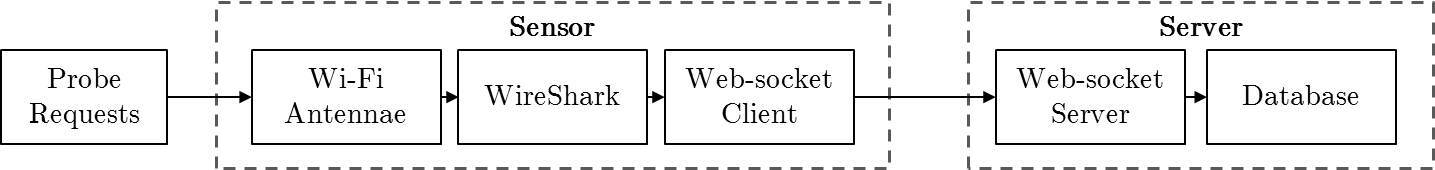
\includegraphics{images/pilot-study-system.jpeg}
  \caption{System diagram showing the data collection process in the pilot study.}
  \label{figure:collection:pilot:schema}
\end{figure*}

\subsection{Locations}
Locations where sensors were installed, volume and speed of probe requests collected by the sensor and total pedestrians manually counted.
The data occupies around 1.8 GB on disk when encoded in text format.
The locations at which the data were collected are shown in Table .
The locations were chosen for their diverse site conditions and unique sources of noise around the potential location of the sensors.
The position of the sensor at these locations with respect to the context is shown the Figure 
We can see that Location 5 is the `cleanest' with one clear stationary source of noise (phone shop) while location 2 is the most complex due to the proximity of seating areas to the sensor.
The sensors were operational through out February and March, while manual counts were conducted in these locations in half hour sessions on at least two different days.
For the purposes of comparing with ground truth, we considered the data from sensors which correspond to the 12 sets of available manual counts.
The schedule of data collection is shown in Figure .

\begin{figure}
  \centering
  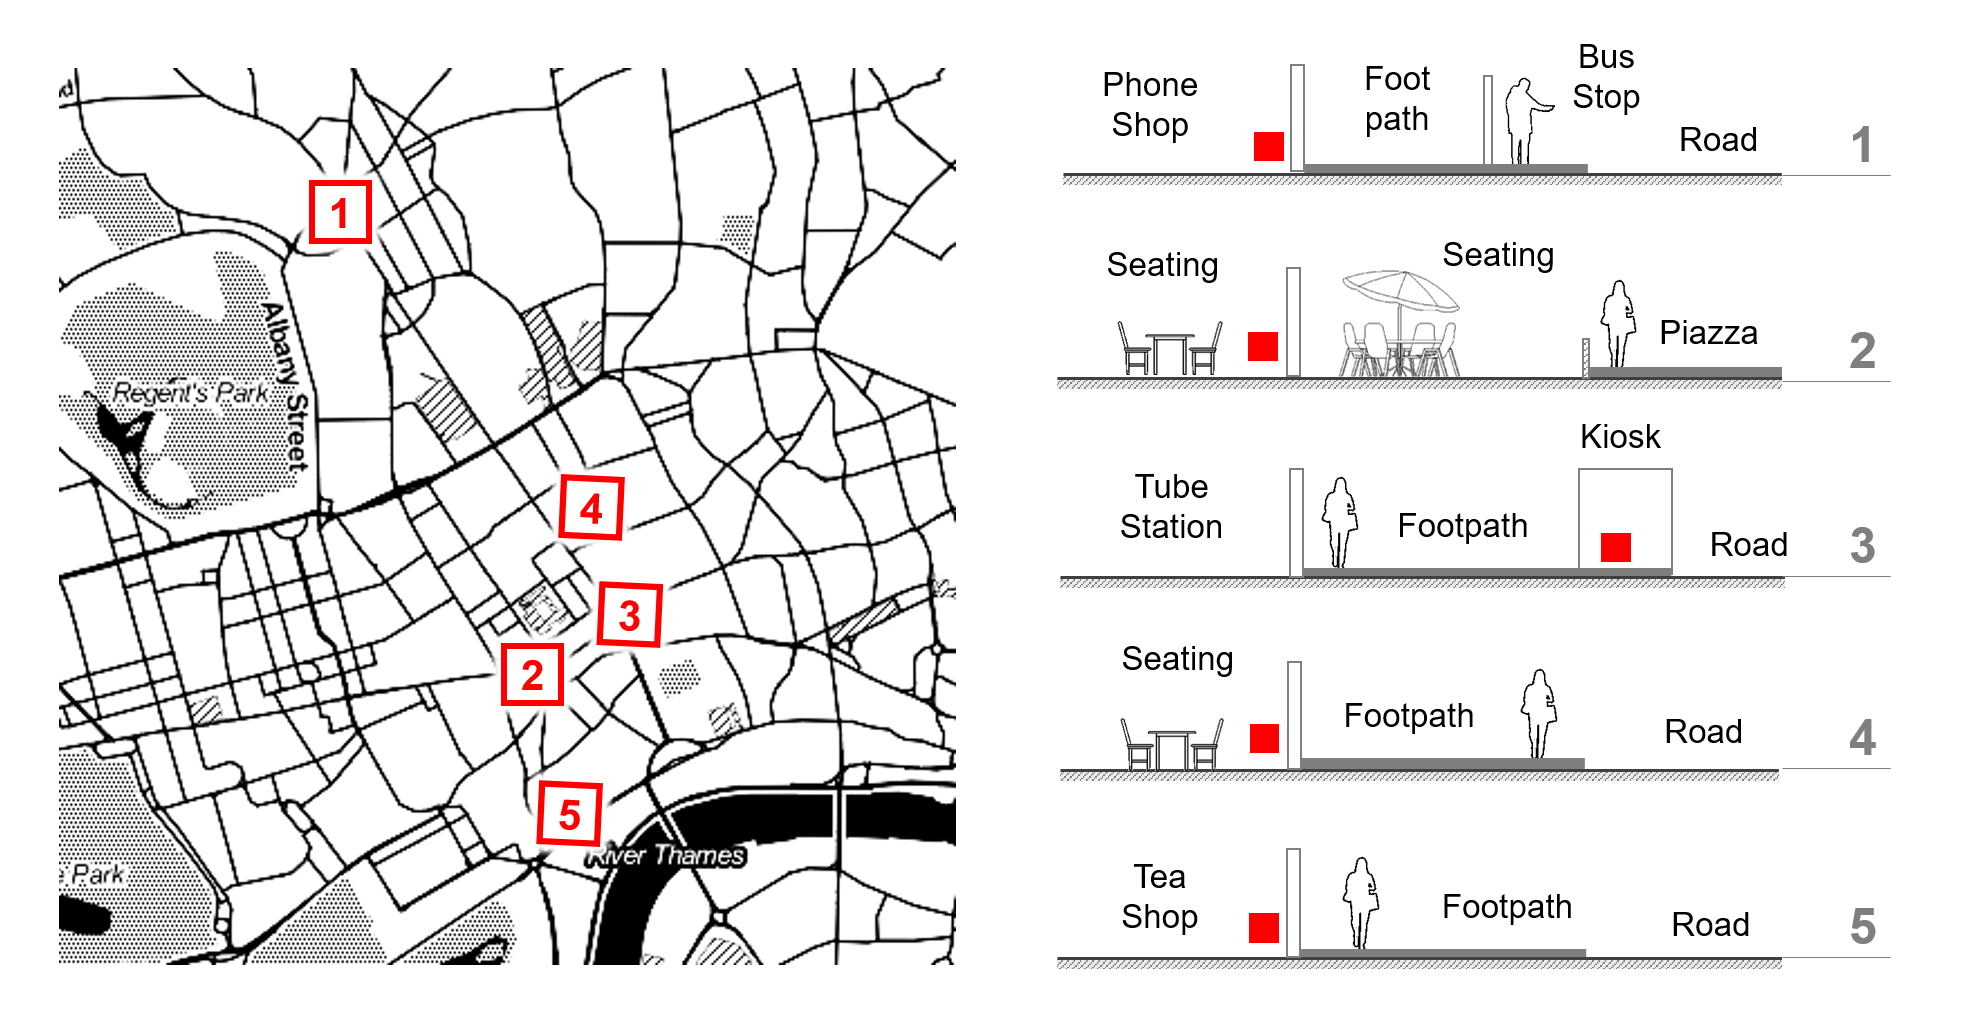
\includegraphics[trim={20 20 20 20},clip, width=\textwidth]{images/pilot-study-locations.png}
  \caption{Pilot study locations in London along with their corresponding sensor installation configurations.}
  \label{figure:literature:tech:timeline}
\end{figure}

\subsection{Data Collection}

\begin{figure*}
  
\includegraphics{images/pilot-study-schedule.png}
  \caption{Outline of the `Medium data toolkit' devised to collect, process, visualise and manage the Wi-Fi probe requests data}
  \label{figure:literature:tech:timeline}
\end{figure*}

\lipsum[1]

\begin{table}
  \footnotesize
  \begin{center}
    \begin{tabular}{clllrr}
      \toprule
        Id & Location & Type & Installation notes & Probes\textsuperscript{*} & Footfall\textsuperscript{**}\\
      \midrule
        \addlinespace[0.2cm]
        1 & Camden St. & Phone Shop & Bus stop in front & 9.9 (297) & 3683 (33)\\
        \addlinespace[0.1cm]
        2 & St.Giles & Restaurant & Seating on both sides & 3.9 (169) & 0346 (05)\\
        \addlinespace[0.1cm]
        3 & Holborn Stn. & Info. Kiosk & Front of station entrance & 4.3 (303) & 2956 (46)\\
        \addlinespace[0.1cm]
        4 & Brunswick & Fast Food & Seating  on one side & 3.4 (210) & 0960 (12)\\
        \addlinespace[0.1cm]
        5 & The Strand & Tea Shop & Phone shop next door & 8.4 (382) & 1969 (21)\\
        \addlinespace[0.05cm]
      \bottomrule
    \end{tabular}
  \end{center}
  \caption{Locations of data collection in the pilot study and the amount of data collected at each locations}
  \label{table:collection:pilot:location}
\end{table}
\marginnote[-1.5cm]{\textit{*something  **somethingelse}}
